% \documentclass[a4paper]{jarticle} % 一般的なスタイルの書き方
\documentclass[a4paper,twocolumn]{ujarticle} % 2段構成のスタイル
%\documentclass[a4paper]{jreport} %卒論原稿はこのスタイル
\setlength{\topmargin}{-2.04cm}%例:上余白を設定
\setlength{\oddsidemargin}{-1.04cm}%例:左余白を1.5cmにする
\setlength{\evensidemargin}{-1.04cm}%例b:左余白を1.5cmにする
\setlength{\textwidth}{18cm}%例:一行の幅を18cmにする
\setlength{\textheight}{25cm}%例:一ページの文章の縦の長さを25cmにする
%\setlength{\textwidth}{45em}%例:一行の文字数を45文字にする(未使用)

%%%%%%%%%%%%%%%%%%%%%%%%%%
%% usepaclagae 群
%%%%%%%%%%%%%%%%%%%%%%%%%%
\usepackage{amsmath,bm} %多次元空間ベクトルRを表記するのに必要
\usepackage{amsfonts}
\usepackage{ascmac} %枠付き文章を表記するのに必
\usepackage{amssymb}
% \mathbb{R}^{l} %表記例
% \usepackage{algorithm}
% \usepackage{algorithmicx}
% \usepackage{algpseudocode}
\usepackage[dvipdfmx]{graphicx}
\usepackage[dvipdfmx]{color}
\usepackage{here} %[hbtp]の代わりに[H]と書きこむと強制的にその場所に図や表を挿入す
\pagestyle{empty}%ページ番号を表示しない

%%%%%%%%%%%%%%%%%%%%%%%%%
\newcommand{\argmax}{\mathop{\rm arg~max}\limits}
\newcommand{\argmin}{\mathop{\rm arg~min}\limits}
%%%%%%%%%%%%%%%%%%%%%%%%%


\makeatletter
\def\@maketitle{%
\begin{center}%
{\LARGE \@title \par}% タイトル
\end{center}%
\begin{flushright}%
{\large \@date}% 日付
\end{flushright}%
\begin{flushright}%%
{\large \@author}% 著者
\end{flushright}%
\par\vskip 1.5em
}
\makeatother
\title{RidgeとLassoの推定} %ここにタイトルを記入すること.
\date{2019年5月8日}
\author{大森 夢拓}

\begin{document}
\maketitle
\section{はじめに}
複雑な非線形構造を内在する現象の分析では,線形モデルや多項式モデルのような特定の関数式で捉えることは難しく,線形モデルではなく非線形モデルで考える必要がある.非線形モデルを推定する方法の一つである正則化法の中でも,本稿ではRidge回帰とLassoを用いた推定を紹介する.また,それらを用いて実際のデータに対して行った計算機実験についても紹介する.
\section{Ridge回帰とLassoの推定}
正則化項のパラメータベクトルの長さの概念を一般化した$L_q$ノルムと呼ばれる正則化項を用いた正則最小2乗法は
\begin{equation}
	S\gamma(w) = \sum_{i=1}^{n}\bigl(
		y_i - \sum_{j=1}^{m} w_j b_j(x_i)
	\bigr)^2 + \gamma \sum_{j=1}^{m} |w_j|^q
	\label{eq:extendLinearRegression}
\end{equation}
のように拡張される.\eqref{eq:extendLinearRegression} が$L_1$ノルムの場合をLasso,$L_2$ノルムの場合をRidge回帰と呼ぶ.
\subsection{Ridge回帰}
線形回帰モデル
\begin{equation}
	y_i=\beta_0 + \beta_1 x_{i1} + \beta_2  x_{i2} + \dots + \beta_p x_{ip} + \epsilon_i, \quad i = 1,2,\dots,n \label{eq:linear_model_origin}
\end{equation}
において,切片を除く回帰係数の2乗和をペナルティ項としてとることで,説明変数$\bm x = (x_1, x_2, \dots , x_p)^{\top}$間の強い相関によって生じる回帰係数の推定値の不安定性を回避する方法である.Ridge推定量の求め方は次のようになる.

各説明変数に関するデータの平均値を$\bar{x}$,中心化したデータを$z_{ij}=x_{ij} - \bar{x}_j$とすると,線形回帰モデル\eqref{eq:linear_model_origin}は次のように変形できる.
\begin{equation}
	\begin{split}
	y_i &= \beta_0 + \beta_1 \bar{x_{i1}} + \beta_2 \bar{x_{i2}} + \dots + \beta_p \bar{x_{ip}} +	\\
	&\quad \beta_1 (x_{i1} - \bar{x_{i1}}) + \beta_2 (x_{i2} - \bar{x_{i2}}) + \dots + \beta_p (x_{ip} - \bar{x_{ip}}) + \epsilon_i, \\
	&i = 1, 2, \dots , n
	\end{split}
	\label{eq:linear_model_centering}
\end{equation}
線形回帰モデル\eqref{eq:linear_model_centering}を,$\beta_0^* = \beta_0 + \beta_1 \bar{x_{i1}} + \dots + \beta_p \bar{x_p}$,成分が全て1のn次元ベクトル $\bm 1 = (1, 1, \dots , 1)^{\top}$,各説明変数の回帰係数からなるp次元ベクトル$\bm{\beta_1} = (\beta_1, \beta_2, \dots , \beta_p)^{\top}$を用いることで次のような行列形式に変形できる.
\begin{equation}
	\begin{split}
		\bm{y} &= \beta_0^* \bm{1} + Z \bm{\beta_1} + \bm{\epsilon}\\
		Z &= \left[
                \begin{array}{ccc}
                z_{11} & \dots & z_{1p} \\
                \dots & z_{ij} & \dots \\
                z_{n1} & \dots & z_{np} \\
                \end{array}
                \right], \quad
                z_{ij} = x_{ij} - \bar{x_j};\\
                &\quad i = 1, \dots, n; \quad
                j = 1, \dots, n
	\end{split}
	\label{eq:linear_model_mat}
\end{equation}
行列形式の線形モデル\eqref{eq:linear_model_mat}より,回帰係数のRidge推定量は,
\begin{equation}
	S\gamma(\beta_0^* , \bm{\beta_1}) = (\bm{y} - \beta_0^* \bm{1} - Z \bm{\beta_1})^{\top} (\bm{y} - \beta_0^* \bm{1} - Z \bm{\beta_1}) + \gamma \bm{\beta_1}^{\top} \bm{\beta_1} 
	\label{eq:ridge_estimate}
\end{equation}
の偏微分による最小化によって,次のような切片の推定量と回帰係数ベクトルのRidge推定量が与えられる.
\begin{equation}
	\hat{\beta_0^*} = \bar{y}, \quad \hat{\bm{\beta_1}} = (Z^{\top}Z + \gamma I_p)^{-1} Z^{\top} \bm{y}.
	\label{eq:ridge_estimate_res}
\end{equation}
以上より,\eqref{eq:linear_model_origin}の切片は$\hat{\beta_0} = \bar{y} - \hat{\beta_1} \bar{x_1} - ... - \hat{\beta_p} \bar{x_p}$の切片と推定されるので,回帰係数ベクトルのリッジ推定量は,$\bm{\beta_1} = (\beta_1, \beta_2, \dots, \beta_p)^{\top}$と,中心化したデータから構成された計画行列Zを用いた$S\gamma(\bm{\beta_1}) = (\bm{y} - Z \bm{\beta_1})^{\top}  (\bm{y} - Z\bm{\beta_1}) + \gamma \bm{\beta_1}^{\top} \bm{\beta_1}$の最小化によって与えられる.
\subsection{Lasso}
線形回帰モデル\eqref{eq:linear_model_origin}において,切片を除く回帰係数の和をペナルティ項としてとることで,パラメーターの一部を完全に0と推定するようなモデルの推定・変数選択を同時に実行できる方法である.切片を除く回帰係数はデータを中心化することによって切片と切り離して測定できるため、
\begin{equation}
        S\gamma(\beta_1, \beta_2, \dots , \beta_p) = \sum_{i=1}^{n} \bigl(
        	y_i - \sum_{j=1}^{p} \beta_j(x_{ij} - \bar{x_j})
        \bigr)^2 + \gamma \sum_{j=1}^{p}|\beta_j|.
\end{equation}
の最小化によって与えられる.ところが,$L_1$正則化項が微分不可能であるため解析的に求めることはできない.
このため,Fu(1998)によるshootingアルゴリズムやEfron et al.(2004)によるLARS(Least Angle Regression) と呼ばれる計算方法が用いられる.

また,ラグランジュの未定乗数法を適用すると、次の様な制約条件つきのパラメータベクトルの最小化と同等になる.
\begin{equation}
	\sum_{i=1}^{n}\bigl(
		y_i - \sum_{j=1}^{m} w_j b_j(x_i)
	\bigr)^2, \quad 制約条件 \sum_{j=1}^{m} |w_j|^q \leq \eta.
\end{equation}
\section{計算機実験}
データセットとしてアメリカのボストン州の住宅価格を,それに影響を与えていると思われる説明変数13個との関係を線形回帰モデルでモデル化した.
データ数は506である.
説明変数は以下の通りである.

\begin{table}[htb]
	\begin{tabular}{ll}
	$x_1$: 犯罪率  & $x_2$: 宅地の割合\\
	$x_3$: 非商用地 &  $x_4$: チャールズ川流域か否か\\
	$x_5$: 窒素酸化物 &  $x_6$: 部屋数\\
	$x_7$: 築年 &  $x_8$: ビジネス地域への距離\\
	$x_9$: ハイウェイアクセス指数 &  $x_{10}$: 固定資産税\\
	$x_{11}$: 生徒と教師の比率 &  $x_{12}$: 有色人種の割合\\
	$x_{13}$: 低所得者の割合\\
	\end{tabular}
\end{table}

通常の最小2乗法と,正則化項の係数をalphaとして0.01, 0.1, 1, 10, 100を値にした5通りにクロス・バリデーション法を用いて決定した値(Ridge回帰:79.43,Lasso:0.16)を合わせた計6通りのRidge回帰,Lassoで回帰係数の推定を行い,それぞれ比較した.この実験結果を図\ref{fig:lr},図\ref{fig:ridge},図\ref{fig:lasso}に示し,Lassoの解パスを図\ref{fig:lasso_path},決定係数の推移を図\ref{fig:score}, 表\ref{tab:score}に示す.

図\ref{fig:lr},図\ref{fig:ridge},図\ref{fig:lasso}より,最小2乗法に比べてalphaが大きくなるにつれて,Ridge回帰では$x_3$〜$x_5$の$\beta$の値が0に向かって縮小しており,Lassoでは全ての値が0に向かって縮小している.特に,Lassoではalpha=100の場合は全ての$\beta$の値が0となっている.これらの結果から,Ridge回帰およびLassoでの正則化項によるペナルティの与えられ方や,Lassoではペナルティによって変数選択が行われていることを確認することができた.

また,図\ref{fig:lasso_path}のLassoの解パスを確認することで,どの説明変数がどの大きさのペナルティによって変数選択が行われているかも確認できた.

最後の図\ref{fig:score},表\ref{tab:score}では,設定したalphaの値における決定係数の推移が確認できるが,今回の実験ではalphaが大きくなるにつれて決定係数が小さくなっていることから,今回のデータではRidge回帰及びLassoの恩恵を受けられなかったことが分かった.

\begin{figure}[H]
    \begin{tabular}{cc}
    	\begin{minipage}{0.5\hsize}
                	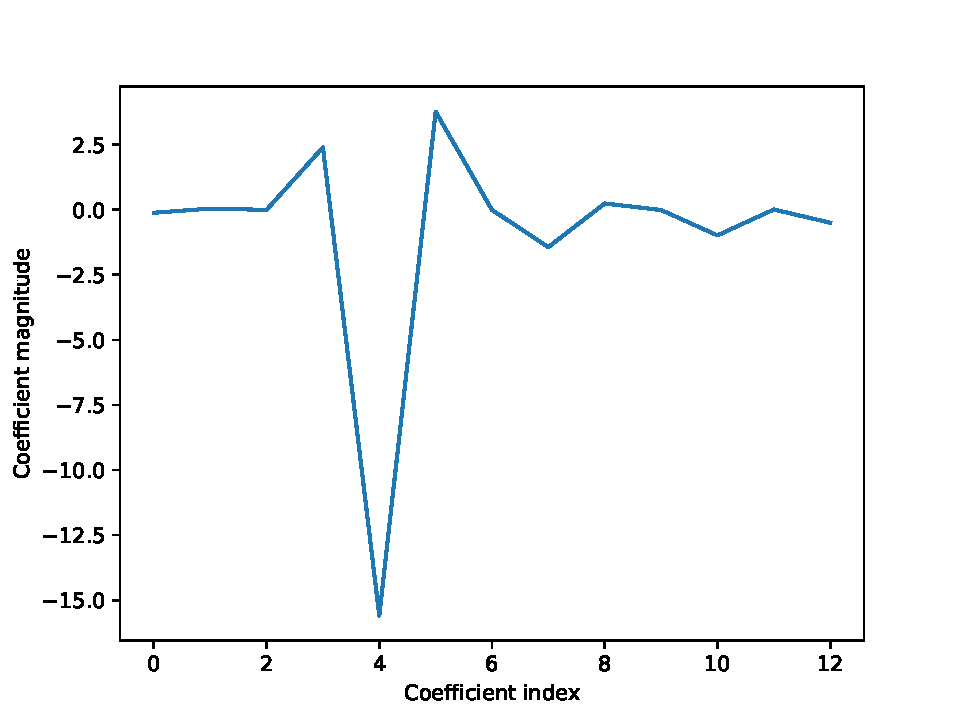
\includegraphics[width=1.0\linewidth]{../img/lr.pdf}
                	\caption{最小2乗法}
               	\label{fig:lr}
    	 \end{minipage}
    	 \begin{minipage}{0.5\hsize}
       		 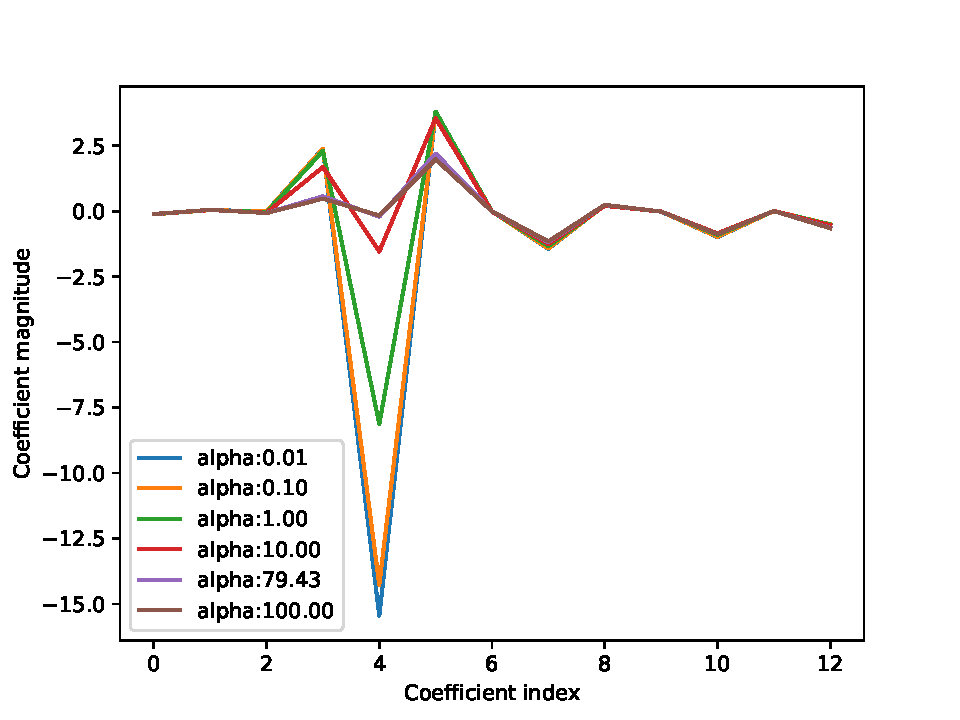
\includegraphics[width=1.0\linewidth]{../img/ridgeCoef.pdf}
    		 \caption{Ridge回帰}
    		 \label{fig:ridge}
    	 \end{minipage}
	     \end{tabular}
\end{figure}

\begin{figure}[H]
    \begin{tabular}{cc}
	 \begin{minipage}{0.5\hsize}
                	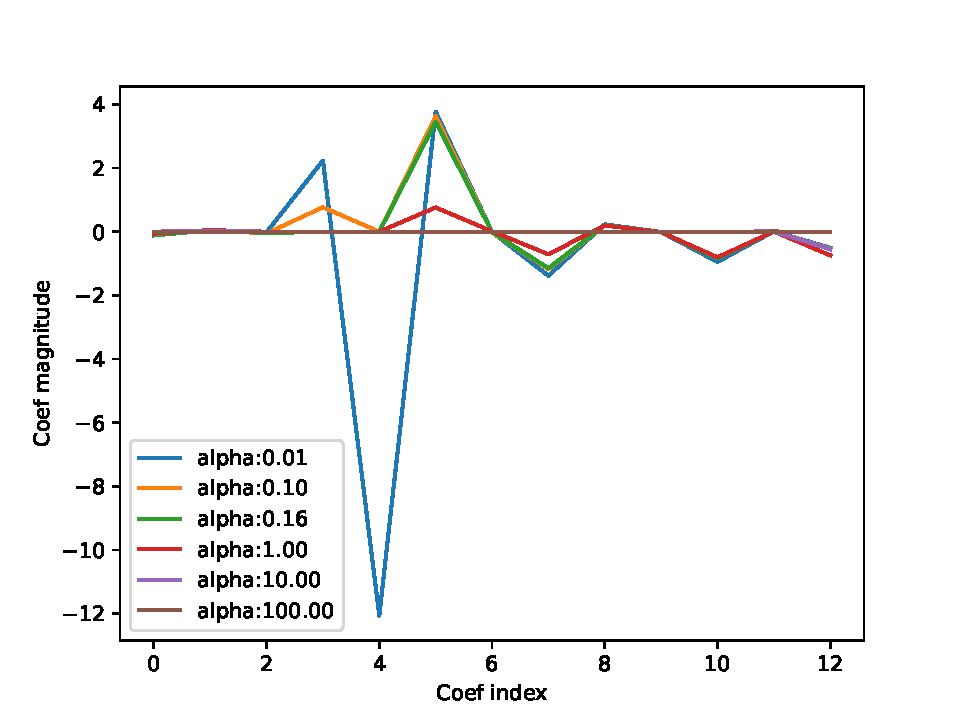
\includegraphics[width=1.0\linewidth]{../img/lassoCoef.pdf}
                	\caption{Lasso}
               	\label{fig:lasso}
    	 \end{minipage}
    	 \begin{minipage}{0.5\hsize}
       		 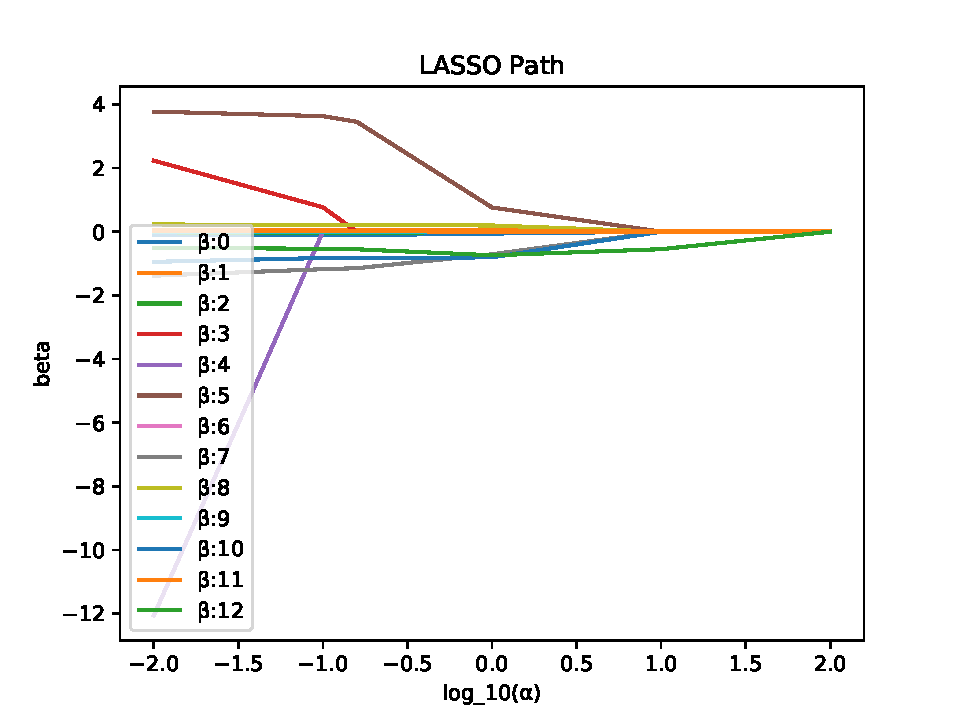
\includegraphics[width=1.0\linewidth]{../img/lassoPath.pdf}
    		 \caption{Lassoの解パス}
    		 \label{fig:lasso_path}
    	 \end{minipage}
	\end{tabular}
\end{figure}

\begin{figure}[H]
    \begin{tabular}{cc}
	  \begin{minipage}{0.5\hsize}
                	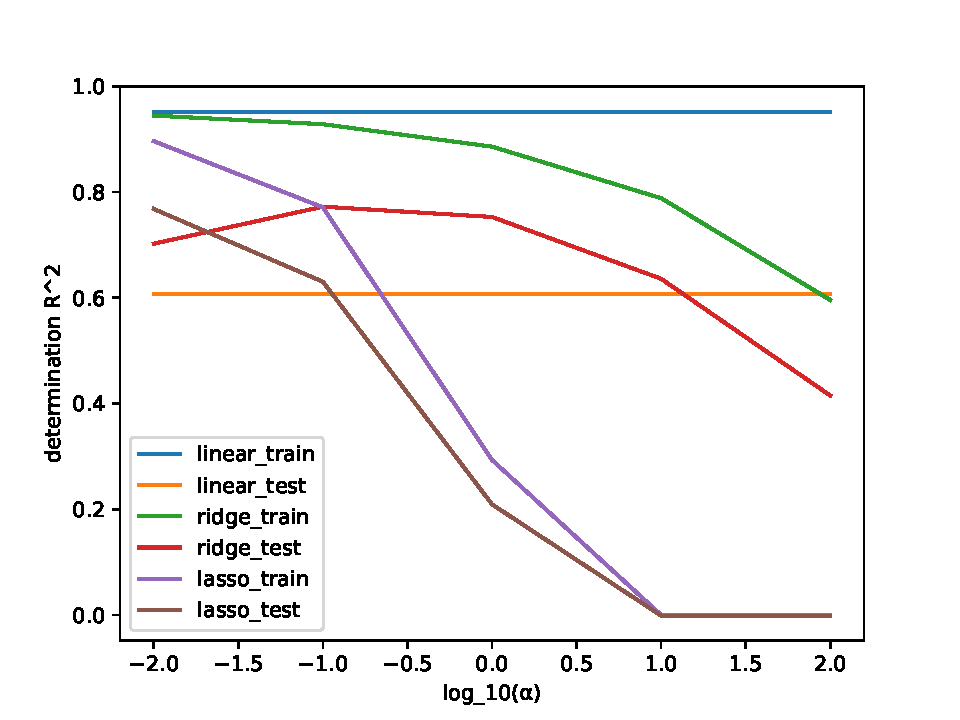
\includegraphics[width=1.0\linewidth]{../img/score.pdf}
                	\caption{決定係数}
               	\label{fig:score}
    	 \end{minipage}
    \end{tabular}
\end{figure}
\begin{table}[H]
	\caption{決定係数の表}
        	\begin{tabular}{|c|c|c|c|c|c|c|c|}
		\hline
        		alpha & 0.01 & 0.1 &0.16 & 1 & 10 & 79 & 100\\ 
		\hline
		\hline
		\multicolumn{8}{|c|}{train} \\
		\hline
		linear & \multicolumn{7}{|c|}{0.77} \\
		\hline
		ridge & 0.77 & 0.77 & & 0.77 & 0.76 & 0.75 & 0.75\\
		\hline
		lasso & 0.77 & 0.76 & 0.76 &0.72 & 0.56 & & 0.25\\
		\hline
		\hline
		\multicolumn{8}{|c|}{test} \\
		\hline
		linear & \multicolumn{7}{|c|}{0.64} \\
		\hline
		ridge & 0.64 & 0.63 & & 0.63 & 0.61 & 0.60 & 0.59\\
		\hline
		lasso & 0.63 & 0.61 & 0.60 &0.55 & 0.40 & & 0.12\\
		\hline
        	\end{tabular}
	\label{tab:score}
\end{table}
\section{まとめ}
Ridge回帰とLassoを中心に,正則化法や非線形回帰モデルについて学ぶことができた.数式だけでなく,Pythonのパッケージを用いた計算機実験による可視化を通して,自分の中でさらにイメージを具体化させることができた.

今後は,Lassoの計算に用いるアルゴリズムを理解して,パッケージを使わずに実装することが課題である.
\begin{thebibliography}{9}
\bibitem{SK} 小西貞則, 『多変量解析入門』. 岩波書店, 2009.
\end{thebibliography}


\end{document}










